\section{Documentação}

Uma documentação bem elaborada proporciona inúmeros benefícios para o desenvolvimento de projetos na área da tecnologia. No caso da \ac{api} desenvolvida em \textit{\gls{.NET}}, a documentação das suas rotas de acesso foi realizada por meio do \textit{\gls{Swagger}}, com o objetivo de facilitar o entendimento de cada rota e sua função no sistema.

A imagem inaugural aborda de maneira específica as rotas correspondentes aos mecanismos de acesso e ao gerenciamento da conta do usuário. Estes \textit{\gls{Endpoints}} podem ser observados com clareza na Figura \ref{RotasAccount}, sendo que cada um é acompanhado por uma exposição elucidativa acerca do propósito subjacente de sua funcionalidade.

\begin{figure}[H]
    \centering
	\caption{Rotas do Usuário}
    \label{RotasAccount}
    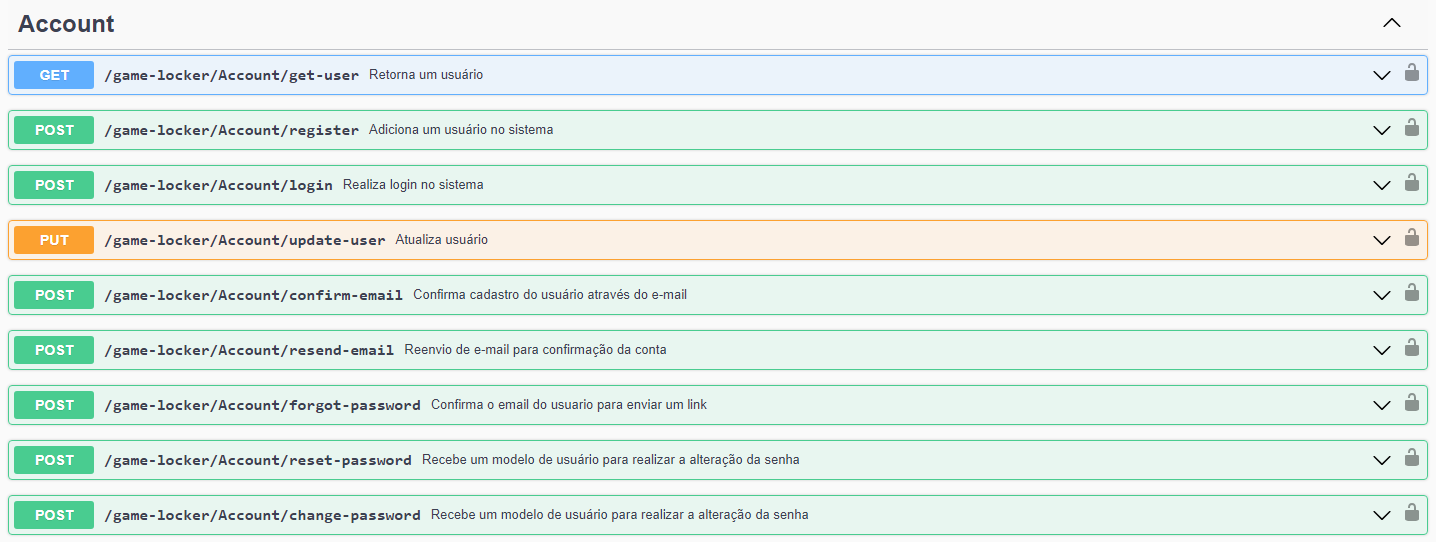
\includegraphics[scale = 0.38]{imagens/arquitetura/rotas_account.png}	
    \fonte{Os Autores}
\end{figure}

A segunda representação gráfica ilustra de maneira distintiva a rota destinada ao acesso a uma \ac{api} externa fornecida pela \textit{\gls{Rawg}}. É imperativo enfatizar que esta invocação à \ac{api} externa ocorre de modo exclusivo no \textit{\gls{Back-end}}, uma precaução tomada em virtude das considerações de segurança inerentes à aplicação. A Figura \ref{RotasApi} proporciona uma visualização precisa dessa rota singular, oferecendo uma compreensão nítida do seu papel e relevância intrínseca no contexto da arquitetura da aplicação.

\begin{figure}[H]
    \centering
	\caption{Rota da API externa}
    \label{RotasApi}
    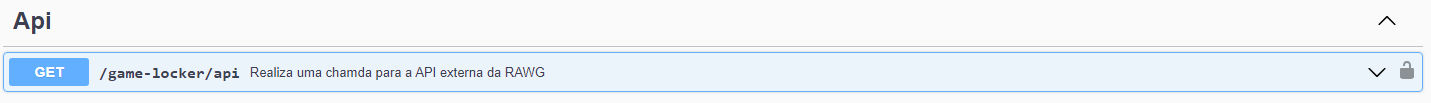
\includegraphics[scale = 0.38]{imagens/arquitetura/rotas_api.png}	
    \fonte{Os Autores}
\end{figure}

A terceira representação gráfica fornece uma visão abrangente de todas as rotas relacionadas às \gls{Review} no âmbito da aplicação. Esta seção assume um papel central na aplicação, demandando, assim, uma ênfase adicional em termos de considerações. A Figura \ref{RotasReview} elucida essas rotas de maneira detalhada, delineando as respectivas funcionalidades que desempenham no contexto do projeto.

\begin{figure}[H]
    \centering
	\caption{Rotas de Review}
    \label{RotasReview}
    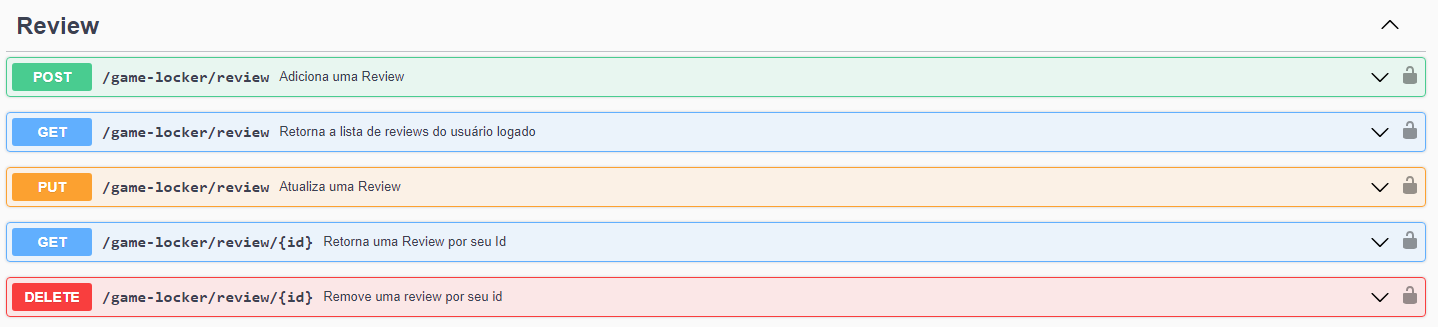
\includegraphics[scale = 0.38]{imagens/arquitetura/rotas_review.png}	
    \fonte{Os Autores}
\end{figure}

A figura \ref{RotasArena} descreve as rotas relacionadas à Arena de Jogos da Aplicação, fornecendo um panorama geral sobre as responsabilidades dessas rotas.

\begin{figure}[H]
    \centering
	\caption{Rotas de Arena}
    \label{RotasArena}
    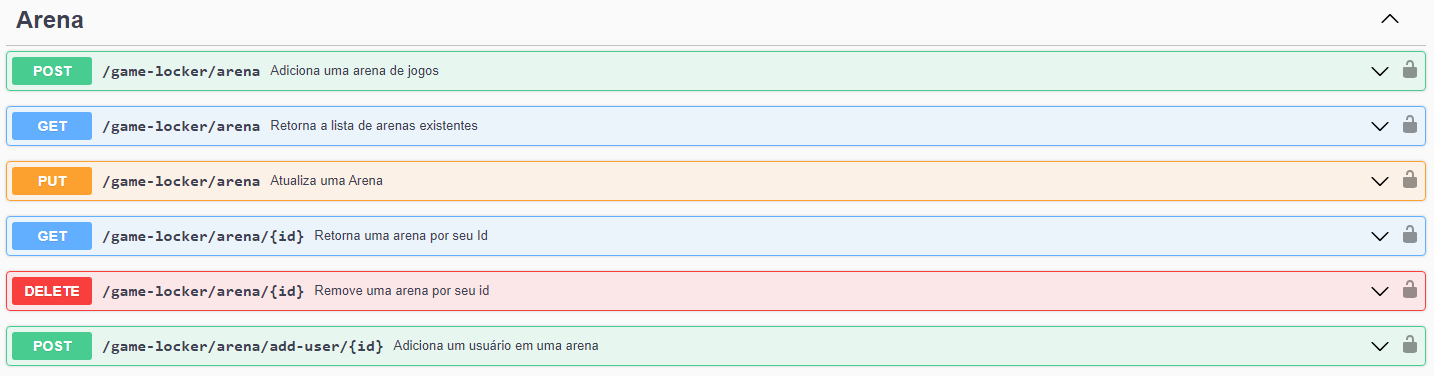
\includegraphics[scale = 0.38]{imagens/arquitetura/rotas_arena.png}	
    \fonte{Os Autores}
\end{figure}

Na figura \ref{RotasPayment} descreve as rotas que interagem diretamente com a \ac{api} do \gls{MercadoPago}, permitindo que as transações sejam realizadas de maneira segura no momento de adesão ao plano premium fornecido na plataforma.

\begin{figure}[H]
    \centering
	\caption{Rotas de Pagamento e Assinaturas}
    \label{RotasPayment}
    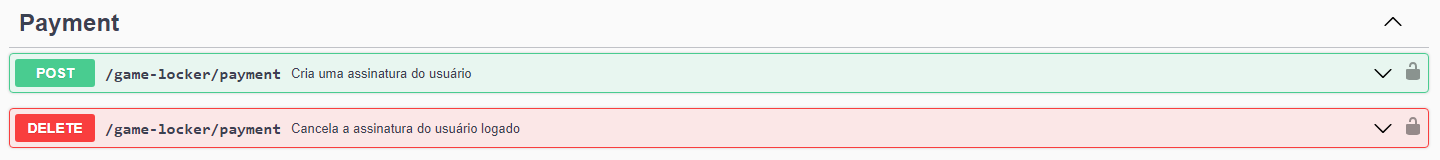
\includegraphics[scale = 0.38]{imagens/arquitetura/rotas_payment.png}	
    \fonte{Os Autores}
\end{figure}

Na Figura \ref{AutenticacaoSwagger}, encontra-se a representação da seção do \gls{Swagger} que assume a responsabilidade pela implementação da autenticação na presente \ac{api}. Importante ressaltar que todas as rotas pertencentes ao \textit{\gls{Back-end}} do projeto, com exceção das rotas de login e cadastro de contas, impõem a necessidade de autenticação para possibilitar o acesso.

\begin{figure}[H]
    \centering
	\caption{Autenticação do Swagger}
    \label{AutenticacaoSwagger}
    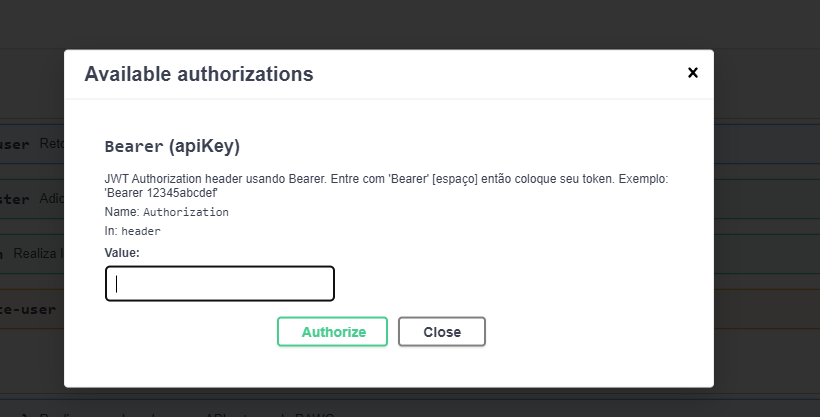
\includegraphics[scale = 0.6]{imagens/arquitetura/rotas_token.png}	
    \fonte{Os Autores}
\end{figure}

Por derradeiro, na Figura \ref{ObjetosEndpoints}, são exibidos em detalhe todos os objetos inerentes às rotas do sistema. Estes objetos carregam a responsabilidade primordial de armazenar e veicular os dados através das interações na aplicação.

\begin{figure}[H]
    \centering
	\caption{Objetos dos Endpoints}
    \label{ObjetosEndpoints}
    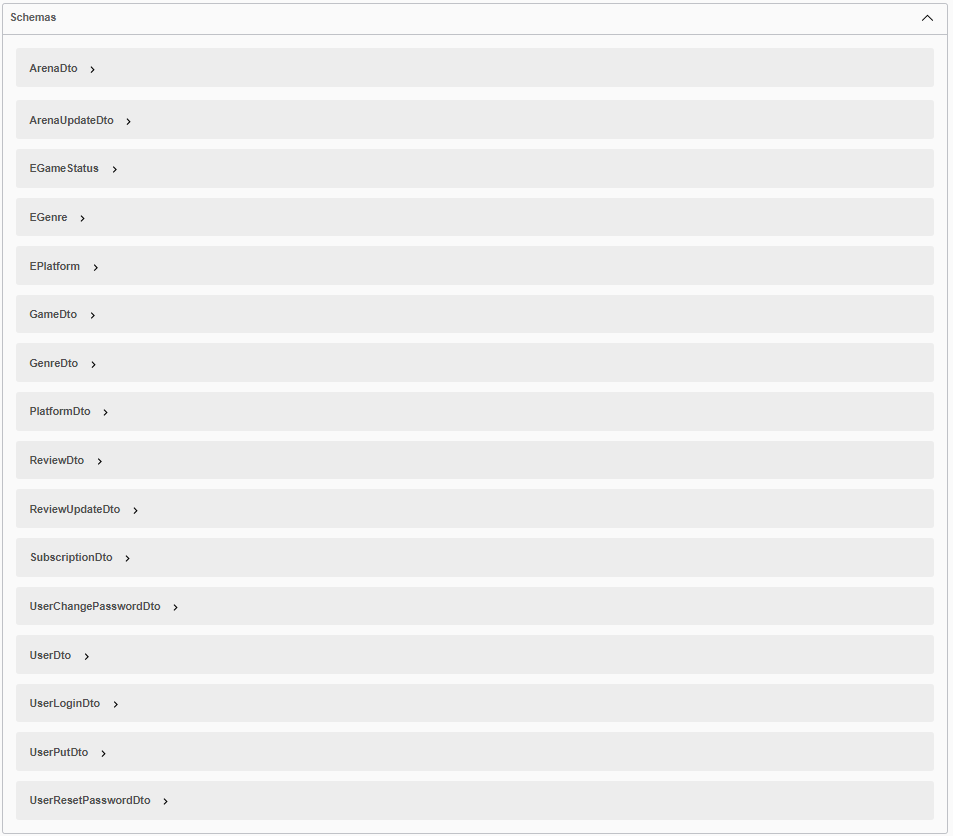
\includegraphics[scale = 0.6]{imagens/arquitetura/rotas_schemas.png}	
    \fonte{Os Autores}
\end{figure}

Para mais informações sobre a \ac{api} do projeto, consultar o link presente no capítulo \ref{LinksProjeto}, que contém este e outros links relevantes.